\documentclass[aspectratio=169]{beamer}
% \pdfpagewidth=1920bp
% \pdfpageheight=1080bp
\setbeamertemplate{navigation symbols}{}
\setbeamertemplate{headline}{} % 无页眉
\setbeamertemplate{bibliography item}{} % 无图标
\usepackage{tikz}
\usepackage{hyperref}
\usepackage{booktabs}

% --- 中文支持(推荐演示用字体:思源黑体/Source Han Sans) ---
\usepackage[UTF8, fontset=windows]{ctex} % 推荐 fontset=windows/mac/ubuntu 以获得更好屏显
% \setCJKmainfont[BoldFont={Source Han Sans SC Bold}, ItalicFont={Source Han Sans SC Light}]{Source Han Sans SC}
% \setCJKsansfont{Source Han Sans SC}
% \setCJKmonofont{Source Code Pro}
% --- Biblatex 设置 ---
\usepackage[
  backend=biber,
  style=keynote,
  citestyle=keynote,
  maxbibnames=1,
  uniquename=false,
  sorting=none
]{biblatex}
\addbibresource{references.bib}
% --- 辅助:左下角参考文献框 ---
\renewcommand*{\bibfont}{\fontsize{5}{6}\selectfont}
\newcommand{\bottomleftrefs}{%
  \begin{tikzpicture}[remember picture,overlay]
    \node[anchor=south west, xshift=1pt, yshift=1pt] at (current page.south west) {%
      \parbox{0.9\linewidth}{
        \setlength{\bibitemsep}{0pt plus 0.3ex}
        \printbibliography[heading=none]
      }
    };
  \end{tikzpicture}%
}

% --- 自定义页脚(含注释说明)---
\setbeamertemplate{footline}{%
  \leavevmode%
  % ----- 左侧:引用区域 -----
  \begin{minipage}[b]{0.70\paperwidth}
    \vspace{0.2em}
    {%
      % 设置引用区域的字体大小和类型
      \fontsize{8}{10}\selectfont % (8pt,10pt 行距)
      \textsf{ % 无衬线字体用于参考文献
        \ifdefined\slidebib
          \slidebib
        \fi
      }
    }
  \end{minipage}%
  \hfill
  % ----- 右侧:版权区域 -----
  \begin{minipage}[b]{0.28\paperwidth}
    \vspace{0.2em}
    \raggedleft
    {%
      % 设置版权字体大小和类型
      \fontsize{9}{11}\selectfont % (9pt,11pt 行距)
      \textrm{ % 衬线字体用于版权
        \textcopyright~2025 Sakura
      }
    }
  \end{minipage}%
}

% 辅助宏:定义每页幻灯片参考文献(每页重置)
\newcommand{\slidebib}{}

%--- 元数据 ---
\title[]{合成数据是否有助于遥感下游任务的能力提升?}
\subtitle{GISLab 2025年暑期短课程}
\author[Sakura]{陈振源}
\institute[ZJU]{浙江大学地球科学学院}
\date{2025\\\small\texttt{bili\_sakura@zju.edu.cn}}

\begin{document}

%--- 封面页 ---
\begin{frame}
  \titlepage
\end{frame}


%--- Slide 1: Outline ---
\begin{refsection}
  \begin{frame}{Outline}
    \begin{itemize}
      \item 1. Introduction to Image Classification using Deep Learning
      \item 2. Traditional Data Augmentation Methods
      \item 3. Generative Models for Data Augmentation
      \item 4. Remote Sensing Dataset for Diaster Events: xBD
    \end{itemize}
    \begin{itemize}
      \item Project - \textbf{Explore whether generated images can benefit image classification}
    \end{itemize}
  \end{frame}
\end{refsection}


\begin{refsection}
  \begin{frame}{Image Classification: Overview}
    \begin{figure}
      \centering
      \includegraphics[height=0.6\textheight]{image_classification_idea.png}
      \caption{\scriptsize Overview of image classification.}
    \end{figure}
    \bottomleftrefs
  \end{frame}
\end{refsection}

\begin{refsection}
  \begin{frame}{Background: Image Classification with Deep Learning}
    \begin{figure}
      \centering
      \begin{minipage}{0.48\linewidth}
        \centering
        \includegraphics[width=\linewidth]{imagenet2.png}
      \end{minipage}\hfill
      \begin{minipage}{0.48\linewidth}
        \centering
        \includegraphics[width=\linewidth]{alexnet.png}
      \end{minipage}
      \caption[]{\scriptsize Left: AlexNet on ILSVRC-2010~\parencite{imagenet2010challenge} \quad Right: Architecture of AlexNet~\parencite{krizhevskyImageNetClassificationDeep2012}.}
    \end{figure}
    \bottomleftrefs
  \end{frame}
\end{refsection}

\begin{refsection}
  \begin{frame}{Architecture Evolution of Image Classification}
    \begin{minipage}{0.48\linewidth}
      {\tiny
      \begin{itemize}
        % \item \textbf{2012: AlexNet} \\
        % \parencite{krizhevskyImageNetClassificationDeep2012}
        % \item \textbf{2016: ResNet} \\
        % \parencite{heDeepResidualLearning2016}
        \item \textbf{NeurIPS 2012: AlexNet (CNN)} \\
        \parencite{krizhevskyImageNetClassificationDeep2012}
        \item \textbf{CVPR 2016: ResNet (CNN)} \\
        \parencite{heDeepResidualLearning2016}
        \item \textbf{ICLR 2021: Vision Transformers (ViT)} \\
        \parencite{dosovitskiyImageWorth16x162020}
        \item \textbf{ICCV 2021: Swin Transformer (ViT)} \\
        \parencite{liuSwinTransformerHierarchical2021}
        \item \textbf{ICML 2021: CLIP (ViT)} \\
        \parencite{radfordLearningTransferableVisual2021}
        \item \textbf{CVPR 2022: MAE (ViT)} \\
        \parencite{heMaskedAutoencodersAre2022}
        \item \textbf{TMLR 2022: CoCa (ViT)} \\
        \parencite{yuCoCaContrastiveCaptioners2022}
      \end{itemize}
      }
    \end{minipage}%
    \hfill
    \begin{minipage}{0.48\linewidth}
      \centering
      \includegraphics[width=0.95\linewidth]{vit.png}
      \scriptsize Overview of Vision Transformer\\\parencite{dosovitskiyImageWorth16x162020}.
    \end{minipage}
    \bottomleftrefs
  \end{frame}
\end{refsection}

% \begin{refsection}
%   \begin{frame}{RemoteCLIP: Vision-Language Foundation Model for Remote Sensing}
%     \begin{figure}
%       \centering
%       \includegraphics[width=0.8\linewidth]{remoteclip.png}
%       \caption{\scriptsize RemoteCLIP~\parencite{liuRemoteCLIPVisionLanguage2024}: A Vision-Language Foundation Model for Remote Sensing.}
%     \end{figure}
%     \bottomleftrefs
%   \end{frame}
% \end{refsection}

\begin{refsection}
  \begin{frame}{Image Classification Dataset: RESISC45}
    \begin{figure}
      \centering
      \includegraphics[width=0.7\linewidth]{RESISC45_part.png}
    \end{figure}
    \scriptsize
    Example images from the RESISC45 remote sensing scene classification dataset~\parencite{Cheng2017}.
    \bottomleftrefs
  \end{frame}
\end{refsection}

\begin{refsection}
  \begin{frame}{Traditional Data Augmentation Methods}
    \begin{itemize}
      \item \textbf{Geometric Transformations:} \textbf{Rotation}, \textbf{Flipping} (horizontal/vertical), \textbf{Scaling}, \textbf{Translation}, \textbf{Cropping}
      \item \textbf{Color Jittering:} Adjusting brightness, contrast, saturation, and hue
      \item \textbf{Noise Injection:} Adding random noise to images
      \item \textbf{Cutout}~\parencite{devriesImprovedRegularizationConvolutional2017}
      \item \textbf{CutMix}~\parencite{yunCutMixRegularizationStrategy2019}
      \item \textbf{Copy-Paste}~\parencite{ghiasiSimpleCopyPasteStrong2021}
    \end{itemize}
    There is also a comprehensive study entitled 'How to train your ViT? Data, Augmentation,  and Regularization in Vision Transformers'~\parencite{steinerHowTrainYour2022}.
    \bottomleftrefs
  \end{frame}
\end{refsection}

\begin{refsection}
  \begin{frame}{Generative Models for Data Augmentation}
    \begin{minipage}{0.7\linewidth}
      % \centering
      \includegraphics[width=0.9\linewidth]{satsyn.png}
    \end{minipage}%
    \hfill
    \begin{minipage}{0.3\linewidth}
      \scriptsize
      SatSyn~\parencite{tokerSatSynthAugmentingImageMask2024} proposes a generative model (diffusion model) to generate both images and corresponding masks for satellite segmentation. The synthetic dataset is used for data augmentation, yielding significant quantitative improvements in satellite semantic segmentation compared to other data augmentation methods.
    \end{minipage}
    \bottomleftrefs
  \end{frame}
\end{refsection}

\begin{refsection}
  \begin{frame}{Generated Text-Image Dataset Improving Image Classification}
    \centering
    \includegraphics[width=0.8\linewidth]{syn_aug_results.png}
    
    % \vspace{0.5em}
    
    \scriptsize
    Synthetic text-image datasets generated by generative models can significantly improve image classification performance, as demonstrated in~\parencite{heSYNTHETICDATAGENERATIVE2022}.
    \bottomleftrefs
  \end{frame}
\end{refsection}

\begin{refsection}
  \begin{frame}{xBD: A Large-Scale Disaster Damage Dataset}
    \centering
    \includegraphics[width=0.85\linewidth]{xbd_samples.png}
    
    \vspace{0.5em}
    \scriptsize
    Pre-disaster imagery (top) and post-disaster imagery (bottom). From left to right: Hurricane Harvey; Joplin tornado; Lower Puna volcanic eruption; Sunda Strait tsunami. Imagery from DigitalGlobe.\\
    \textbf{xBD}~\parencite{guptaCreatingXBDDataset2019}
    \bottomleftrefs
  \end{frame}
\end{refsection}

\begin{refsection}
  \begin{frame}{xBD: Global Coverage of Disaster Types}
    \centering
    \includegraphics[width=0.85\linewidth]{xbd_global.png}
    
    \vspace{0.5em}
    \scriptsize
    Disaster types and disasters represented in xBD around the world.\\
    \textbf{xBD}~\parencite{guptaCreatingXBDDataset2019}
    \bottomleftrefs
  \end{frame}
\end{refsection}

\begin{refsection}
  \begin{frame}{Project Assignment: Overview}
    \textbf{Project: Can Generated Images Improve Remote Sensing Image Classification?}
  
    \vspace{0.7em}
    \textbf{Objective:}\\
    Investigate whether combining real images and generated images can improve remote sensing image classification.

    \vspace{1em}
    \textbf{Pipeline:}\\
    In this project, you will experiment with three different training settings to evaluate the impact of generated data:
    \begin{enumerate}
      \item \textbf{Real Dataset Only:} Train the classification model using only real images from the xBD dataset.
      \item \textbf{Generated Dataset Only:} Train the model using only synthetic images generated by commercial generative models.
      \item \textbf{Combined Dataset:} Train the model using both real and generated images together.
    \end{enumerate}
    Compare the classification performance across these three settings to analyze the effect of synthetic data.

    \bottomleftrefs
  \end{frame}
\end{refsection}
  
%--- Slide: Dataset ---
\begin{refsection}
  \begin{frame}{Project Assignment: Dataset}
    \textbf{Dataset: xBD Disaster Damage Dataset}
    \begin{itemize}
      \item Use the \textbf{xBD} remote sensing disaster dataset.
      \item The dataset includes \textbf{6 disaster classes}.
      \item For each class, use \textbf{100 real images} (total: 600 real images).
    \end{itemize}
    \bottomleftrefs
  \end{frame}
  \end{refsection}
  
  %--- Slide: Generative Models ---
  \begin{refsection}
    \begin{frame}{Project Assignment: Generative Models}
      \textbf{Image Generation:}
      \begin{itemize}
        \item We consider generated images as the result of \textbf{text-guided image editing}: for each case, you input a \textbf{pre-event image} and a \textbf{text description} (e.g., "flooded", "collapsed building"), and the model yields a generated (post-event) image.
        \item Use commercial generative models such as \textbf{GPT-4o Image Generation(GPT-Image-1)}~\parencite{gptimage1}, \textbf{Gemini-2}~\parencite{gemini2}, or \textbf{SeedEdit 3.0}~\parencite{wang2025seedit} to create synthetic images for each disaster class.
      \end{itemize}
      \bottomleftrefs
    \end{frame}
  \end{refsection}
  
  
  %--- Slide: Classification Models ---
  \begin{refsection}
  \begin{frame}{Project Assignment: Classification Models}
    \textbf{Recommended Baseline Models:}
    \begin{itemize}
      \item \textbf{OpenAI CLIP}~\parencite{radfordLearningTransferableVisual2021}~\href{https://hf-mirror.com/openai/clip-vit-base-patch16}{\textcolor{blue}{- models}}
      \item \textbf{RemoteCLIP}~\parencite{liuRemoteCLIPVisionLanguage2024}~\href{https://hf-mirror.com/MVRL/remote-clip-vit-base-patch32}{\textcolor{blue}{- models}}
      \item \textbf{Git-RSCLIP}~\parencite{text2earth2025}~\href{https://hf-mirror.com/lcybuaa/Git-RSCLIP-base}{\textcolor{blue}{- models}}
    \end{itemize}
    \vspace{0.5em}
    All of the above follow ViT configurations. For code and tutorials:
    \begin{itemize}
      \item \href{https://github.com/huggingface/transformers/blob/main/examples/pytorch/contrastive-image-text/README.md}{\textcolor{blue}{CLIP training example}}
      \item \href{https://github.com/NielsRogge/Transformers-Tutorials/tree/master/VisionTransformer}{\textcolor{blue}{ViT tutorials}}
      \item For more Remote Sensing Foundation Models, ref to ~\href{https://hf-mirror.com/collections/MVRL/remote-sensing-foundation-models-664e8fcd67d8ca8c03f42d00}{\textcolor{purple}{huggingface collection}.}
      \item The latest strong baseline RSFM 'SkySense-O'~\parencite{zhuSkySenseOOpenWorldRemote2025}. \href{https://github.com/zqcrafts/SkySense-O}{\textcolor{blue}{GitHub}}

    \end{itemize}
    \bottomleftrefs
  \end{frame}
  \end{refsection}
  
  %--- Slide: Data Augmentation Protocol ---
  \begin{refsection}
  \begin{frame}{Project Assignment: Data Augmentation Protocol}
    \begin{itemize}
      \item For each disaster class, generate \textbf{1$\times$--4$\times$} synthetic images (i.e., 100, 200, 300, or 400 synthetic images per class).
      \item Explore and compare different ratios of real to synthetic images (e.g., 1:1, 1:2, 1:3, 1:4).
      \item The augmented dataset for each class will range from \textbf{200 to 500 images}.
    \end{itemize}
    \bottomleftrefs
  \end{frame}
  \end{refsection}
  
  %--- Slide: Evaluation ---
  \begin{refsection}
  \begin{frame}{Project Assignment: Evaluation}
    \textbf{Evaluation:}
    \begin{itemize}
      \item Use \textbf{standard accuracy}, \textbf{F1 score}, and \textbf{confusion matrix} to measure performance.
      \item Always evaluate on a \textbf{held-out real (unseen) test set}.
      \item Include \textbf{curve or bar plots} comparing classification performance across different real:synthetic ratios.
    \end{itemize}
    \bottomleftrefs
  \end{frame}
  \end{refsection}
  

% \begin{refsection}
%   \begin{frame}{Baseline Models for Scene Classification}
%     \textbf{Scene Image Classification:}
%     \begin{itemize}
%       \item \textbf{OpenAI CLIP}~\parencite{radfordLearningTransferableVisual2021}~\href{https://hf-mirror.com/openai/clip-vit-base-patch16}{\textcolor{blue}{- models}}
%       \item \textbf{RemoteCLIP}~\parencite{liuRemoteCLIPVisionLanguage2024}~\href{https://hf-mirror.com/MVRL/remote-clip-vit-base-patch32}{\textcolor{blue}{- models}}
%       \item \textbf{Git-RSCLIP}~\parencite{text2earth2025}~\href{https://hf-mirror.com/lcybuaa/Git-RSCLIP-base}{\textcolor{blue}{- models}}
%     \end{itemize}
%     All of above follow ViT configuration where we can use following~\href{https://github.com/huggingface/transformers/blob/main/examples/pytorch/contrastive-image-text/README.md}{\textcolor{blue}{(code)}}~for continuing CLIP training or ~\href{https://github.com/NielsRogge/Transformers-Tutorials/tree/master/VisionTransformer}{\textcolor{blue}{(code)}}~ for fine-tuning on classification task.
%     For more Remote Sensing Foundation Models, ref to ~\href{https://hf-mirror.com/collections/MVRL/remote-sensing-foundation-models-664e8fcd67d8ca8c03f42d00}{\textcolor{purple}{huggingface collection}.}
%     \bottomleftrefs
%   \end{frame}
%   \end{refsection}



\begin{refsection}
  \begin{frame}[plain]
    \vfill
    \centering
    {\Huge \textbf{Appendix}}
    \vfill
  \end{frame}
\end{refsection}

  %--- Slide: Datasets for Text-to-Image Generation ---
  \begin{refsection}
    \begin{frame}{Additonal Text-Image Remote Sensing Datasets}
      \textbf{Text-to-Image Generation:}
      \begin{itemize}
        \item \textbf{RSICD}~\parencite{lu2017exploring}: Remote Sensing Image Captioning Dataset with 10,921 images and five captions per image.
        \item \textbf{RSICap}~\parencite{hu2023rsgpt}: High-quality dataset with 2,585 human-annotated image-caption pairs.
        \item \textbf{UCM-Captions}~\parencite{qu2016deep}: Derived from the UC Merced Land Use Dataset, containing 2,100 images with five captions each.
        \item \textbf{RESISC45}~\parencite{Cheng2017}: It is a publicly available benchmark for REmote Sensing Image Scene Classification (RESISC), created by Northwestern Polytechnical University (NWPU). This data set contains 31 500 images, covering 45 scene classes with 700 images in each class.
      \end{itemize}
      \bottomleftrefs
    \end{frame}
  \end{refsection}

\begin{refsection}
  \begin{frame}{Generative Modeling}
    \begin{figure}
      \centering
      \includegraphics[width=0.8\linewidth]{learning_to_generate_data.png}
      \caption{\scriptsize Illustration of generative modeling~\parencite{CVPR2023Tutorial}.}
    \end{figure}
    \bottomleftrefs
  \end{frame}
  \end{refsection}
  
  % --- Slide 2: Timeline of Generative Models ---
  \begin{refsection}
  \begin{frame}{Timeline of Generative Models}
    \begin{figure}
      \centering
      \includegraphics[width=0.95\linewidth]{genai_timeline.png}
      \caption{\scriptsize Timeline of key developments in generative models~\parencite{dengPPTAdvancedNueralNetwork2024}.}
    \end{figure}
    \bottomleftrefs
  \end{frame}
  \end{refsection}
  
  
  
  \begin{refsection}
  \begin{frame}{Background: Diffusion Models}
  
    \begin{figure}
      \begin{minipage}{0.95\linewidth}
        \footnotesize
        \textbf{Denoising diffusion models consist of two processes:}
        \begin{itemize}
          \item A forward diffusion process that gradually adds noise to the input.
          \item A reverse denoising process that learns to generate data by denoising.
        \end{itemize}
      \end{minipage}
      \vspace{2em}
  
      \centering
      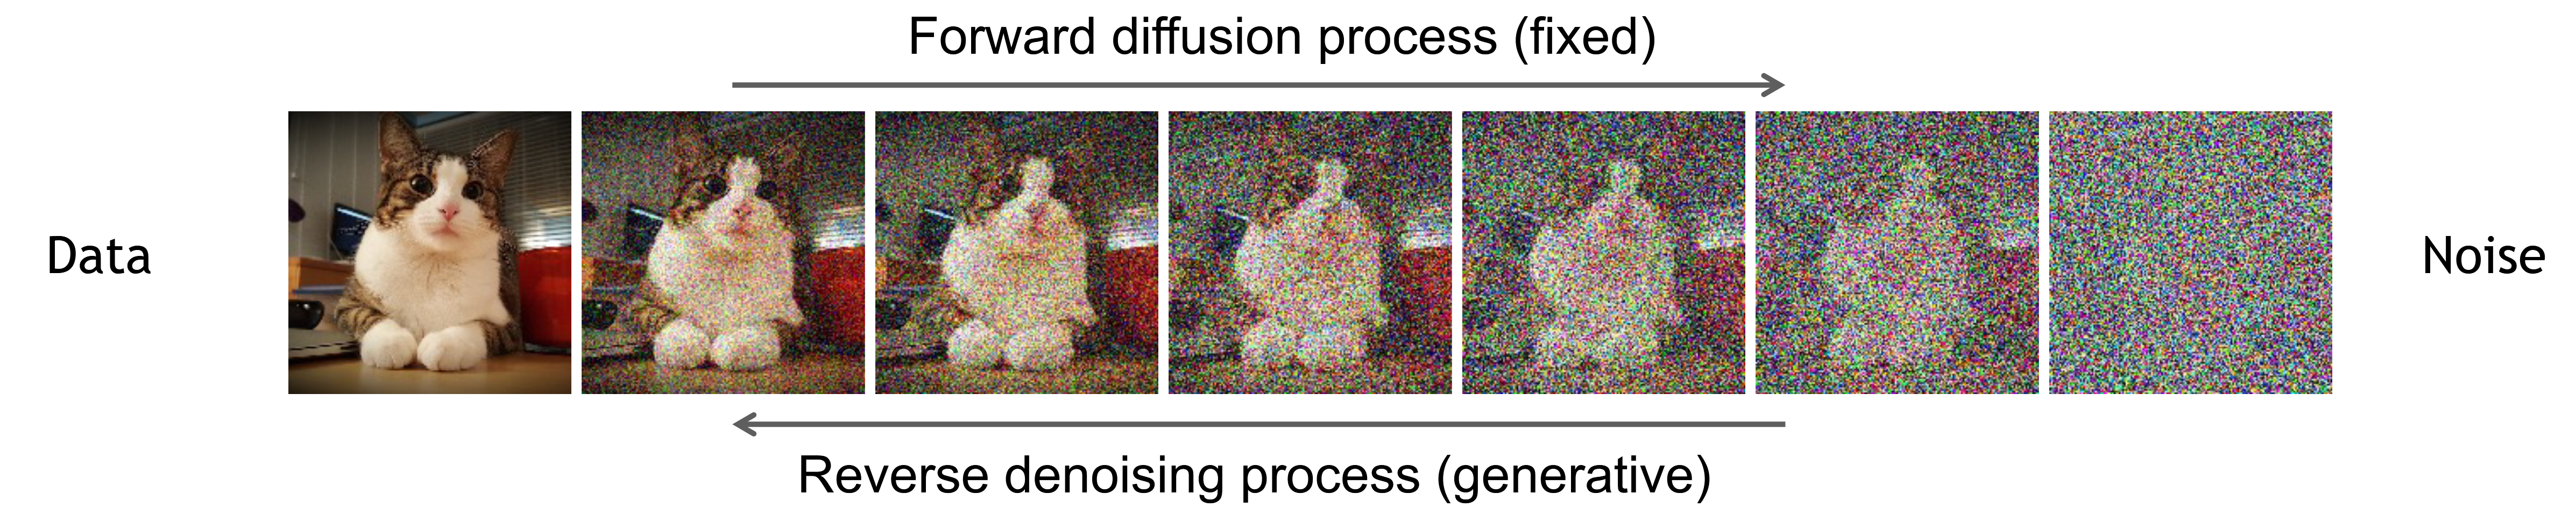
\includegraphics[width=1.0\linewidth]{diffusion_high_level.png}
  
      \caption[]{\scriptsize Diffusion models generate data through iterative denoising~\parencite{sohl2015deep,ho2020denoising}.}
    \end{figure}
  
    \bottomleftrefs
  \end{frame}
  \end{refsection}
  
  % --- Slide 4: Preliminaries of Diffusion Models ---
  \begin{refsection}
  \begin{frame}{Diffusion Models: Forward and Reverse Processes}
    \footnotesize
    \textbf{Forward (Diffusion) Process:}
    \begin{align*}
      q(\mathbf{x}_t \mid \mathbf{x}_{t-1}) &= \mathcal{N}(\mathbf{x}_t; \sqrt{1-\beta_t}\,\mathbf{x}_{t-1}, \beta_t \mathbf{I}) \\
      q(\mathbf{x}_{1:T} \mid \mathbf{x}_0) &= \prod_{t=1}^T q(\mathbf{x}_t \mid \mathbf{x}_{t-1}) \\
      &\text{Equivalently,  } 
      \mathbf{x}_t = \sqrt{\bar{\alpha}_t}\,\mathbf{x}_0 + \sqrt{1-\bar{\alpha}_t}\,\boldsymbol{\epsilon}, \quad \boldsymbol{\epsilon} \sim \mathcal{N}(\mathbf{0}, \mathbf{I})
    \end{align*}
  
    \footnotesize
    \textbf{Reverse (Denoising) Process:}
    \begin{align*}
      p_\theta(\mathbf{x}_{t-1} \mid \mathbf{x}_t) &= \mathcal{N}(\mathbf{x}_{t-1}; \boldsymbol{\mu}_\theta(\mathbf{x}_t, t), \Sigma_\theta(\mathbf{x}_t, t)) \\
      p_\theta(\mathbf{x}_{0:T}) &= p(\mathbf{x}_T) \prod_{t=1}^T p_\theta(\mathbf{x}_{t-1} \mid \mathbf{x}_t)
    \end{align*}
    \scriptsize
    where $\mathbf{x}_0$ is the data, $\beta_t$ is the noise schedule, and $\bar{\alpha}_t = \prod_{s=1}^t (1-\beta_s)$. $p(\mathbf{x}_T) = \mathcal{N}(\mathbf{0}, \mathbf{I})$.
  
    \scriptsize
    \textbf{Diffusion models generate data by learning to reverse a gradual noising process.}~\parencite{sohl2015deep,ho2020denoising}
    \bottomleftrefs
  \end{frame}
  \end{refsection}
  
  \begin{refsection}
  \begin{frame}{Diffusion Models: Training and Inference}
    \footnotesize
    \textbf{Training Objective:}
    \begin{align*}
      \mathcal{L}_{\mathrm{simple}} = \mathbb{E}_{\mathbf{x}_0, \boldsymbol{\epsilon}, t} \left[ \left\| \boldsymbol{\epsilon} - \boldsymbol{\epsilon}_\theta(\sqrt{\bar{\alpha}_t}\mathbf{x}_0 + \sqrt{1-\bar{\alpha}_t}\boldsymbol{\epsilon}, t) \right\|^2 \right]
    \end{align*}
    where $\boldsymbol{\epsilon} \sim \mathcal{N}(\mathbf{0}, \mathbf{I})$, $\bar{\alpha}_t = \prod_{s=1}^t (1-\beta_s)$.
  
    \vspace{0.5em}
    \textbf{Inference (Sampling):}
    \begin{itemize}
      \item Start from pure noise: $\mathbf{x}_T \sim \mathcal{N}(\mathbf{0}, \mathbf{I})$
      \item For $t = T, \ldots, 1$:
        \begin{itemize}
          \item Predict noise: $\boldsymbol{\epsilon}_\theta(\mathbf{x}_t, t)$
          \item Compute mean: $\boldsymbol{\mu}_\theta(\mathbf{x}_t, t)$
          \item Sample: $\mathbf{x}_{t-1} \sim \mathcal{N}(\boldsymbol{\mu}_\theta(\mathbf{x}_t, t), \Sigma_\theta(\mathbf{x}_t, t))$
        \end{itemize}
      \item Repeat until $\mathbf{x}_0$ (generated sample)
    \end{itemize}
  
    \vspace{0.5em}
    \scriptsize
    \textbf{Training:} Minimize the simplified objective~\parencite{ho2020denoising}.\\
    \textbf{Inference:} Iteratively denoise from random noise to generate data.
    \bottomleftrefs
  \end{frame}
  \end{refsection}
  
  %--- Slide 5: Application in Remote Sensing Image Generation: DiffusionSat, CRS-Diff, Text2Earth ---
  
  \begin{refsection}
    \begin{frame}{Application in Remote Sensing Image Generation: Text2Earth}
      \begin{figure}
        \centering
        \includegraphics[width=0.9\linewidth]{text2earth.png}
        \caption[]{\scriptsize Text2Earth: Foundation model for text-driven Earth observation~\parencite{text2earth2025}.}
      \end{figure}
      \bottomleftrefs
    \end{frame}
  \end{refsection}
  
  \begin{refsection}
    \begin{frame}{Text2Earth: Example Results}
      \begin{figure}
        \centering
        \includegraphics[width=0.9\linewidth]{text2earth_results.png}
        \caption[]{\scriptsize Example results generated by Text2Earth~\parencite{text2earth2025}.}
      \end{figure}
      \bottomleftrefs
    \end{frame}
  \end{refsection}
  
  \begin{refsection}
  \begin{frame}{Application in Remote Sensing Image Generation: CRS-Diff}
    \begin{figure}
      \centering
      \includegraphics[width=0.9\linewidth]{crsdiff.png}
      \caption[]{\scriptsize CRS-Diff: Controllable remote sensing image generation framework~\parencite{tang2024crsdiff}.}
    \end{figure}
    \bottomleftrefs
  \end{frame}
  \end{refsection}
  
  \begin{refsection}
  \begin{frame}{CRS-Diff: Example Results}
    \begin{figure}
      \centering
      \includegraphics[width=0.9\linewidth]{crsdiff_results.png}
      \caption[]{\scriptsize Example results generated by CRS-Diff~\parencite{tang2024crsdiff}.}
    \end{figure}
    \bottomleftrefs
  \end{frame}
  \end{refsection}
  
  
  %--- Slide 6a: DiffusionSat Framework ---
  \begin{refsection}
  \begin{frame}{DiffusionSat: Framework Overview}
    \begin{figure}
      \centering
      \includegraphics[width=0.9\linewidth]{diffusionsat.png}
      \caption[]{\scriptsize DiffusionSat: A generative foundation model for satellite imagery~\parencite{diffusionset2024}.}
    \end{figure}
    \bottomleftrefs
  \end{frame}
  \end{refsection}
  
  %--- Slide 6b: DiffusionSat for Super-Resolution ---
  \begin{refsection}
  \begin{frame}{DiffusionSat: Super-Resolution Results}
    \begin{figure}
      \centering
      \includegraphics[width=0.9\linewidth]{diffusionsat_sr_results.png}
      \caption[]{\scriptsize Example results: DiffusionSat for multi-spectral super-resolution~\parencite{diffusionset2024}.}
    \end{figure}
    \bottomleftrefs
  \end{frame}
  \end{refsection}
  
  %--- Slide 6c: DiffusionSat for Inpainting ---
  \begin{refsection}
  \begin{frame}{DiffusionSat: Inpainting Results}
    \begin{figure}
      \centering
      \includegraphics[width=0.9\linewidth]{diffusionsat_inpainting_results.png}
      \caption[]{\scriptsize Example results: DiffusionSat for remote sensing image inpainting~\parencite{diffusionset2024}.}
    \end{figure}
    \bottomleftrefs
  \end{frame}
  \end{refsection}

 


\end{document}